%%%%%%%%%%%%%%%%%%%%%%%%%%%%%%%%%%%%%%%%%
% Short Sectioned Assignment
% LaTeX Template
% Version 1.0 (5/5/12)
%
% This template has been downloaded from:
% http://www.LaTeXTemplates.com
%
% Original author:
% Frits Wenneker (http://www.howtotex.com)
%
% License:
% CC BY-NC-SA 3.0 (http://creativecommons.org/licenses/by-nc-sa/3.0/)
%
%%%%%%%%%%%%%%%%%%%%%%%%%%%%%%%%%%%%%%%%%

%----------------------------------------------------------------------------------------
%	PACKAGES AND OTHER DOCUMENT CONFIGURATIONS
%----------------------------------------------------------------------------------------

\documentclass[paper=a4, fontsize=11pt]{scrartcl} % A4 paper and 11pt font size

\usepackage[T1]{fontenc} % Use 8-bit encoding that has 256 glyphs
\usepackage{fourier} % Use the Adobe Utopia font for the document - comment this line to return to the LaTeX default
\usepackage[english]{babel} % English language/hyphenation
\usepackage{amsmath,amsfonts,amsthm} % Math packages
\usepackage{graphicx}
\usepackage{float}
\graphicspath{ {./images/} }
\usepackage{lipsum} % Used for inserting dummy 'Lorem ipsum' text into the template
\usepackage{wrapfig}
\usepackage{sectsty} % Allows customizing section commands
\allsectionsfont{\centering \normalfont\scshape} % Make all sections centered, the default font and small caps

\usepackage{fancyhdr} % Custom headers and footers
\pagestyle{fancyplain} % Makes all pages in the document conform to the custom headers and footers
\fancyhead{} % No page header - if you want one, create it in the same way as the footers below
\fancyfoot[L]{} % Empty left footer
\fancyfoot[C]{} % Empty center footer
\fancyfoot[R]{\thepage} % Page numbering for right footer
\renewcommand{\headrulewidth}{0pt} % Remove header underlines
\renewcommand{\footrulewidth}{0pt} % Remove footer underlines
\setlength{\headheight}{13.6pt} % Customize the height of the header

\numberwithin{equation}{section} % Number equations within sections (i.e. 1.1, 1.2, 2.1, 2.2 instead of 1, 2, 3, 4)
\numberwithin{figure}{section} % Number figures within sections (i.e. 1.1, 1.2, 2.1, 2.2 instead of 1, 2, 3, 4)
\numberwithin{table}{section} % Number tables within sections (i.e. 1.1, 1.2, 2.1, 2.2 instead of 1, 2, 3, 4)

\setlength\parindent{0pt} % Removes all indentation from paragraphs - comment this line for an assignment with lots of text

%----------------------------------------------------------------------------------------
%	TITLE SECTION
%----------------------------------------------------------------------------------------

\newcommand{\horrule}[1]{\rule{\linewidth}{#1}} % Create horizontal rule command with 1 argument of height

\title{	
\normalfont \normalsize 
\textsc{IIT Kharagpur} \\ [25pt] % Your university, school and/or department name(s)
\horrule{0.5pt} \\[0.4cm] % Thin top horizontal rule
\huge Internship Assignment \\ % The assignment title
\horrule{2pt} \\[0.5cm] % Thick bottom horizontal rule
}

\author{Soumyadeep Mukherjee} % Your name

\date{\normalsize\today} % Today's date or a custom date

\begin{document}

\maketitle % Print the title

%----------------------------------------------------------------------------------------
%	PROBLEM 1
%----------------------------------------------------------------------------------------
internship-application@lists.andrew.cmu.edu
\section{Common Assignment}


\subsection{Rotations}
\begin{enumerate}
\item Question 1
\begin{enumerate}
\item Euler Angles:
\begin{itemize}
\item Advantage: More human understandable and intuitive and good to reduce into individual degrees of freedom.
\item Disadvantage: Ambiguity in representation and Gimbal Lock i.e. in lost degree of freedom in boundary cases of +/- 90 degrees. Also, trigonometric functions are slower to calculate than arithmetic.
\end{itemize}
\item Unit Quaternions:
\begin{itemize}
\item Advantage: More compact representation and avoids Gimbal Lock.
\item Disadvantage: Less Intuitive to understand and complicated mathematics. Also, representation of translation with rotation with quaternions is not elegant.
\end{itemize}
\item Rotation Matrix
\begin{itemize}
\item Advantage: All transformations can be represented and the mathematics is easy to understand.
\item Disadvantage: Order of rotation with respect to axis is important to be considered. Multiple representations of same rotation in matrix form. Redundant Representation.
\end{itemize}
\item Axis/Angle Representation
\begin{itemize}
\item Advantage: Very intuitive to understand.
\item Disadvantage: Applying the interpolation in rotation using this is difficult. Number of mathematical operations to perform rotation in this representation is more making it slow.
\end{itemize}
\end{enumerate}
Git Repo Link for further Questions - 
\item Question 2
\begin{align}
R^{a} = 
\begin{bmatrix}
0.353553 &-0.866025  &0.353553 \\
0.612372  &0.5  &0.612372 \\
-0.707107 &0  &0.707107
\end{bmatrix}
\end{align}
\begin{align}
R^{b} = 
\begin{bmatrix}
1        &-0         &0 \\
0       &0.5  &0.866025 \\
0 &-0.866025       &0.5
\end{bmatrix}
\end{align}
\item Question 3
\begin{align}
q^{a} = 
\begin{matrix}
0.800103 &-0.191342 &0.331414 &0.46194
\end{matrix}
\end{align}
\begin{align}
q^{b} = 
\begin{matrix}
0.866025 &-0.5 &0 &0
\end{matrix}
\end{align}
No, Quaternions are not unique representations of rotations. There are two representations of a quaternion, itself and it's negation.
\item Question 4
\begin{align}
q^{c} = 
\begin{matrix}
0.597239 &-0.565758 &0.0560427 &0.565758
\end{matrix}
\end{align}
\begin{align}
q^{d} = 
\begin{matrix}
0.597239 &-0.565758 &0.517982 &0.234345
\end{matrix}
\end{align}
No, they are not same since quaternion multiplication is not commutative.
\item Question 5
\begin{align}
q^{f} = 
\begin{matrix}
0.800103 &-0.191342 &0.331414 &0.46194
\end{matrix}
\end{align}
From (1.3) and (1.7),
\begin{center}$q^{a} = q^{f}$\end{center}

\end{enumerate}
\pagebreak


\subsection{Planning Concepts}

\begin{itemize}
\item Question 1

The distinction between constraints and objectives is that a constraint is a design target that must be met for the design to be successful. In contrast, an objective is a design target where more (or less) is better. 
However, constraints can often be converted into objectives if needed to solve the optimization problem like in Lagrangian functions, the constraints are added to the objective to create a new objective function which is solved for new constraints obtained.

\item Question 2

Homotopy classes of trajectories arise due to presence of obstacles in an environment. Two trajectories connecting the same start and goal coordinates are in the same homotopy class if they can be smoothly deformed into one another without intersecting any obstacle in the environment, otherwise they are in different homotopy classes.
 
In motion planning, it is important to distinguish between trajectories of different homotopy classes, as well as identify the different homotopy classes in an environment (e.g., trajectories that go left around a circle in two dimensions versus right) so that planning of the path constrained to different classes can be done differently and efficiently and also to avoid certain homotopy classes which are not feasible.

Also, a study of homotopy classes ensures a mathematical representation for applying constraints and solving for trajectories within a class along with searching for a trajectory with least cost path becomes simpler due to the classification into classes.

\item Question 3

Motion Planning can be represented as an optimization problem with constraints. Constraints are important to reduce the search space for solution trajectories/paths and these constraints are propagated by using sensing information from environment. This set of information from environment got from interaction with environment is called information gain.

Information gain is the data/information about the surroundings obtained from sensors on a robot which are reduced to constraints for motion planning. Presence of these constraints allows better decisions for motion planning as it can give the necessary data to classify homotopy classes and apply constraints to solve the optimization problem of motion planning. 
\item Question 4

D* Lite repeatedly determines shortest paths between the current vertex of the robot and the goal vertex as the edge costs of a graph change while the robot moves towards the goal vertex making it a deterministic algorithm unlike RRT* that grows a tree rooted at the starting configuration by using random samples from the search space. 

RRT* propagates trees randomly sampling nodes and adding them to node set but in situations where the environment and weight of the edges change, RRT* cannot give an optimal solution and will need to recompute the whole search space for the new set of edge weights.However, D* Lite does not make any assumptions about how the edge costs change, whether they go up or down, whether they change close to the current vertex of the robot or far away from it, or whether they change in the world or only because the robot revised its initial estimates. 

\end{itemize}

\section{Perception}
\subsection{Plane Segmentation}

\paragraph{}
\text{Git Repository for Code:}

\begin{figure}[b]
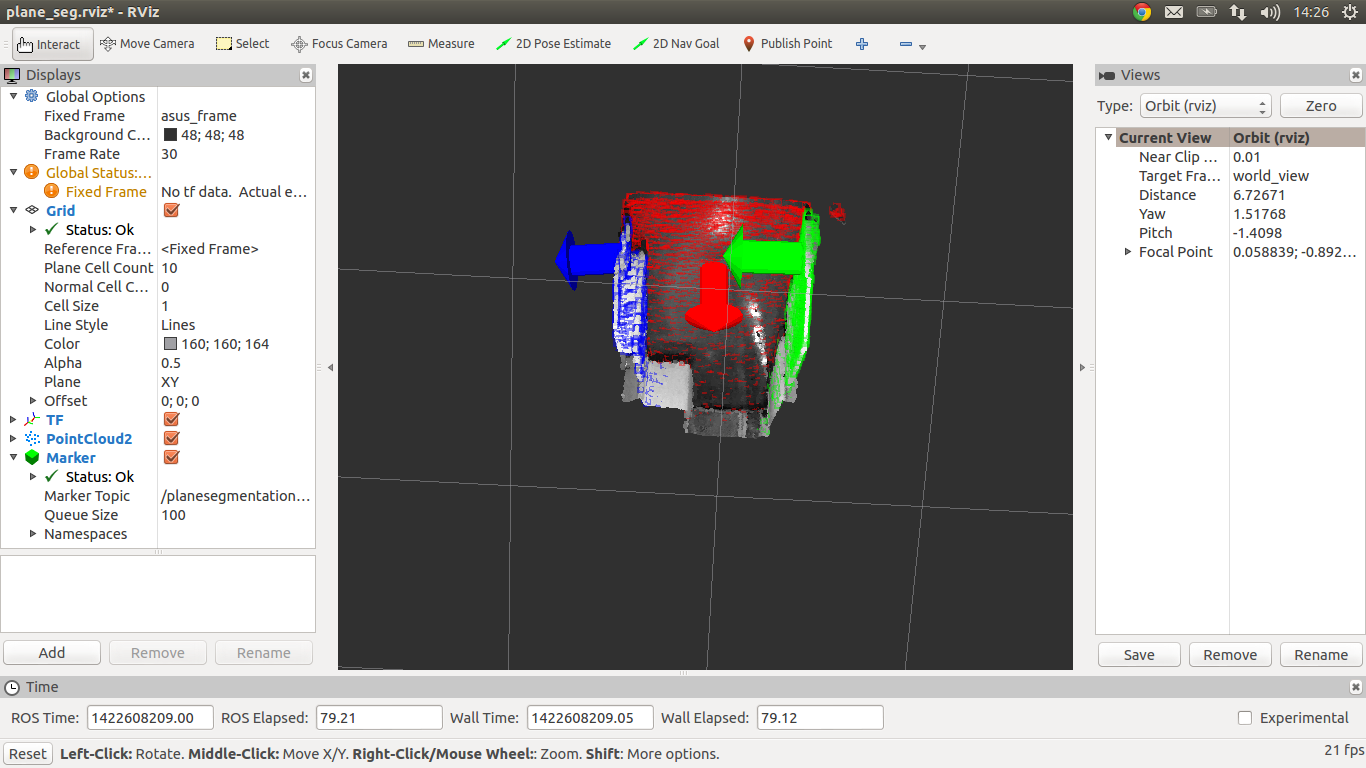
\includegraphics[scale = 0.33,bb = 0 0 0 0]{screenshot.png}
\caption{Screen-shot}
\end{figure}

\paragraph{Approach}
I passed the coefficients calculated for every plane to the visualizing function and then calculated the slope of the normal and plotted them on the plane.
\end{document}